\documentclass[11pt,a4paper]{article}
\usepackage[margin=21mm]{geometry}
\usepackage[T1]{fontenc}
\usepackage{lmodern,microtype,booktabs,tabularx,tikz}
\usetikzlibrary{arrows.meta,positioning}
\usepackage[hidelinks]{hyperref}
\definecolor{ink}{HTML}{183D51}
\definecolor{pale}{HTML}{EBF3F6}
\newcommand{\planversion}{\input{VERSION}}
\setlength{\parindent}{0pt}
\setlength{\parskip}{5pt}
\title{HLA pangenome: a three-day research sprint\\\large High-level plan, v\planversion}
\author{Robert Hoehndorf, Dawn, and Hassan}
\date{15 September 2026}
\begin{document}
\maketitle
\vspace{-1.5em}

\section*{1. The question and the intended outcome}
\textbf{Does a diverse HLA graph improve the recovery and typing of HLA alleles
from short reads, and how much reference diversity is needed?}
We will compare the same 1000 Genomes samples against hg38 and our graph,
using experimental HLA types to assess accuracy. The graph starts from 610
haplotypes; adding Korea and CRC brings the planned panel above 700.
The panel emphasises Asian diversity and includes non-Asian HPRC donors.

\textbf{Three-day outcome:} a working comparison on a independently typed
sample set, a first comparison matrix, error and cost analyses, and initial haplotype
and bundle results. Completion of each analysis depends on data readiness and
measured cluster throughput. The schedule assumes concurrent work by Robert, Dawn, Hassan, and
agents, with access to the cluster and existing data.

\begin{figure}[h!]
\centering
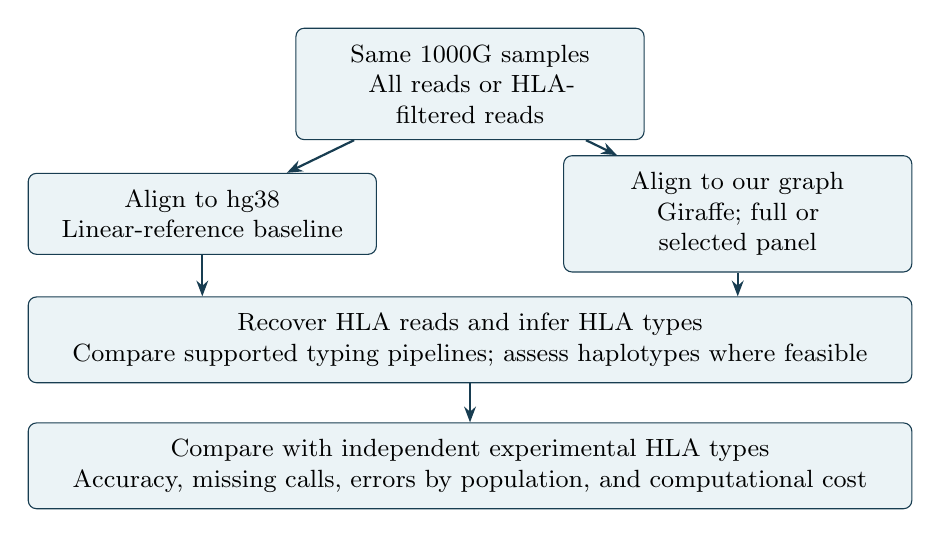
\begin{tikzpicture}[
 box/.style={draw=ink,rounded corners=3pt,fill=pale,align=center,
 text width=4.0cm,minimum height=1.0cm,font=\small,inner sep=6pt},
 arr/.style={-{Stealth[length=2mm]},thick,draw=ink}]
\node[box] (reads) at (0,0) {Same 1000G samples\\All reads or HLA-filtered reads};
\node[box] (linear) at (-3.4,-1.65) {Align to hg38\\Linear-reference baseline};
\node[box] (graph) at (3.4,-1.65) {Align to our graph\\Giraffe; full or selected panel};
\node[box,text width=10.8cm] (type) at (0,-3.25) {Recover HLA reads and infer HLA types\\Compare supported typing pipelines; assess haplotypes where feasible};
\node[box,text width=10.8cm] (eval) at (0,-4.85) {Compare with independent experimental HLA types\\Accuracy, missing calls, errors by population, and computational cost};
\draw[arr] (reads) -- (linear);
\draw[arr] (reads) -- (graph);
\draw[arr] (linear) -- (type.north -| linear.south);
\draw[arr] (graph) -- (type.north -| graph.south);
\draw[arr] (type) -- (eval);
\end{tikzpicture}
\caption{Core experiment. Graph construction and truth-data preparation proceed
in parallel. Experimental labels are used only for evaluation.}
\end{figure}

\section*{2. Keep the first comparison small}
\textbf{Build and check.} Consolidate the assembly panel, build or reuse the HLA
graph, and select an initial pilot of approximately 12--20 available, independently typed
individuals spanning represented populations. Exclude their own assemblies and
close relatives from the graph. Use the pilot to fix the pipeline and then launch a larger held-out cohort
as soon as cluster throughput permits.

\textbf{Compare and explain.} Begin with hg38 versus the full eligible graph and
a shared read set. Then test whether HLA filtering preserves the calls while
reducing cost. Start two compatible HLA typers and add the third in parallel: HLA*LA, T1K,
and SpecHLA. Compare calls at the resolution supported by the experimental assay,
count missing calls, and inspect discordant cases.

\newpage
\section*{3. Three-day timeline: parallel work, early compute}
Plan for agent-assisted implementation at approximately one conventional week
per day, as a working assumption. The critical path is data access, graph
construction/indexing, and cluster runs. The team will decide task assignments.

\renewcommand{\arraystretch}{1.12}
\begin{tabularx}{\textwidth}{@{}p{1.0cm}XX@{}}
\toprule
Day & Concurrent workstreams & Checkpoint and output \\
\midrule
\textbf{1} & Panel QC, graph build/indexes, and subset jobs; experimental
truth, read extraction, and three typer wrappers; scoring, inference prototype,
and experiment manifest.
& First hours: verify data, exclusions, and one end-to-end sample. Launch pilot
and expensive graph jobs immediately; submit bulk runs once the pilot passes.
Leave the cluster processing overnight. \\
\addlinespace
\textbf{2} & Mapping and subset runs; typing and paired evaluation; error
review and inference validation. Expand job arrays, test the prototype, and
analyse existing bundles while compute runs.
& First accuracy/cost comparison; full matrix submitted where resources allow.
Freeze settings before held-out evaluation. Test matched long reads if already
available. Schedule failed-job retries overnight. \\
\addlinespace
\textbf{3} & Complete runs, inspect discordant
calls, analyse population effects and subset sizes, assess haplotype and bundle
results, and write the report.
& Versioned graph, workflows, comparison matrix, uncertainty estimates,
error examples, and exploratory figures. Identify unfinished compute and the
specific evidence needed next. \\
\bottomrule
\end{tabularx}

\textbf{Execution rule.} Agents prepare code, manifests, tests, and reports
concurrently; cluster arrays handle heavy computation. Give each output directory
one owner. Share read-only indexes and cache extraction. Measure a representative
job on day 1, then set concurrency and cohort size from actual memory, runtime,
storage, and queue capacity.

\section*{4. Target comparison matrix}
\begin{tabularx}{\textwidth}{@{}p{3.0cm}X@{}}
\toprule
Axis & Planned conditions \\
\midrule
Reference & hg38; full eligible graph; subsets of 4, 8, 16, 32 individuals. \\
Read input & All reads; HLA-filtered reads plus every unmapped read and mates. \\
HLA typer & HLA*LA, T1K, SpecHLA, using each tool's supported inputs. \\
Selection & Read-guided donor subsets and random controls. Test blockwise
haplotype selection separately if indexes are ready~\cite{personal}. \\
\bottomrule
\end{tabularx}

Prioritise full graph versus hg38, then filtering, then subset size and selection.
Whole-individual subsets retain both available haplotypes; the cited method
selects haplotypes locally in blocks. Avoid duplicate runs when a typer receives
identical reads and realigns them internally.

\textbf{Fallbacks follow compute.} If Korea/CRC indexing is delayed, start with
the available donor-excluded panel and add the expanded graph when ready.
If all-read mapping is expensive, complete it on a smaller paired cohort while
filtered runs continue. Report the actual panel, samples, and completed cells
for every comparison.

\newpage
\section*{5. Assessment: realistic and worth pursuing?}
\textbf{My recommendation is to pursue it.} The existing assembly panel and
analysis work provide a strong starting point. With agents working concurrently,
three days is a credible target for a substantial first benchmark and exploratory
results. Completion is conditional on data readiness and measured compute time.
Assessing rare alleles and population-specific effects depends on the number
of independent, experimentally typed samples available.

\textbf{The strongest scientific question is the value of added diversity.}
HLA graphs already exist~\cite{hlala}. This study becomes compelling if the
expanded panel improves difficult calls, reduces errors in underrepresented
populations, reconstructs additional sequence, or lowers cost. Compare panels
with and without Korea/CRC while controlling panel size to identify what these
additions contribute. A larger graph alone provides a resource; measured benefit
provides the stronger research argument.

\textbf{The hardest step is connecting graph alignment to HLA inference.}
Many typers realign recruited reads to their own references. Their comparison
therefore tests read recruitment. A direct graph-inference experiment requires
an inference stage that uses graph alignments. Assign an agent workstream to
prototype it immediately, validate it on known sequences, and report its results
separately from established typers. Keep both routes so the benchmark progresses
while inference development proceeds.

\textbf{The decisive controls are independent truth and donor exclusion.}
Remove evaluation donors and close relatives from the graph. Match output
resolution to the experimental assay~\cite{truth}; retain ambiguous and missing
calls. Review the paired errors before interpreting an accuracy difference.
Use the pilot for debugging and the held-out samples for evaluation.

\section*{6. Extensions to start in parallel}
\textbf{Haplotypes and long reads.} Infer supported sequences within individual
HLA genes first. Short reads provide local phase information; extended MHC
phasing requires longer links or explicit reference-panel assumptions. I expect
accurate long reads to help most with full-gene reconstruction and phasing.
Test available matched individuals with SpecImmune and HLAminer, controlling
coverage and scoring resolution. Mark absent datasets as dependencies.

\textbf{Bundle classification.} Start from the existing bundle analyses on day 1
or 2. Cluster shared sequence segments without using HLA labels, then measure
recovery of known types on held-out donors. This is a worthwhile exploratory
result. The more ambitious question is whether clusters capture peptide-binding
similarity or structural features beyond conventional HLA groups. Compare
binding-site sequences first; use independent binding evidence as it becomes
available. Population frequencies give context; phenotype associations need
individual-level outcomes and ancestry adjustment.

\textbf{Day 3 decision.} Expand the most reproducible accuracy, cost, or biological
finding. If typing performance is equivalent, examine efficiency and sequence
coverage. If the graph-inference prototype is promising, define its next
validation set. Publish a clear account of completed comparisons and outstanding
compute, together with a prioritised next experiment.

\vspace{-0.5em}
\begin{thebibliography}{3}\small\setlength{\itemsep}{0pt}
\bibitem{personal} Sir\'en J et al. Personalized pangenome references (2024).
\href{https://doi.org/10.1038/s41592-024-02407-2}{Nature Methods, doi:10.1038/s41592-024-02407-2}.
\bibitem{hlala} Dilthey Lab. \href{https://github.com/DiltheyLab/HLA-LA}{HLA*LA: graph-based HLA typing and supported inputs}.
\bibitem{truth} Gourraud P-A et al. HLA diversity in the 1000 Genomes dataset (2014).
\href{https://doi.org/10.1371/journal.pone.0097282}{PLOS ONE, doi:10.1371/journal.pone.0097282}.
\end{thebibliography}
\end{document}
